%%%%%%%%%%%%%%%%%%%%%%%%%%
%%% author : Yamada. T %%%
%%% made for TH series %%%
%%%%%%%%%%%%%%%%%%%%%%%%%%

\documentclass[b5paper,10pt,fleqn] {ltjsarticle}

\usepackage[margin=10truemm]{geometry}

\usepackage{pict2e, graphicx}
\usepackage{tikz}
\usetikzlibrary{intersections,calc,arrows.meta}

\usepackage{amsmath, amssymb, amsthm}
\usepackage{ascmac}
\usepackage{comment}
\usepackage{empheq}
\usepackage[shortlabels,inline]{enumitem}
\usepackage{fancybox}
\usepackage{fancyhdr}
\usepackage{here}
\usepackage{lastpage}
\usepackage{listings, jvlisting}
\usepackage{fixdif}

\usepackage{stmaryrd}
\usepackage[listings]{tcolorbox}
%\usepackage{ascolorbox}
\usepackage{titlesec}
\usepackage{ulem}
\usepackage{url}
\usepackage{verbatim}
\usepackage{wrapfig}
\usepackage{xcolor}
\usepackage{luatexja-ruby}
\usepackage{varwidth}
\usepackage[version=3]{mhchem}
\usepackage{wrapfig}


\usepackage{physics2}
	\usephysicsmodule{ab}
	\usephysicsmodule{ab.braket}
	\usephysicsmodule{ab.legacy}
	%\usephysicsmodule{braket}
	\usephysicsmodule{diagmat}
	\usephysicsmodule{xmat}
	\usephysicsmodule{nabla.legacy}
	\usephysicsmodule{qtext.legacy}

\usepackage[ISO]{diffcoeff}
\difdef { f, s } { D }
{ op-symbol = \mathrm{D} }


\newcommand{\mctext}[1]{\mbox{\textcircled{\scriptsize{#1}}}}
\newcommand{\ctext}[1]{\textcircled{\scriptsize{#1}}}
\newcommand{\ds}{\displaystyle}
\newcommand{\comb}[2]{{}_{#1}\mathrm{C}_{#2}}
\newcommand{\hs}{\hspace}
\newcommand{\vs}{\vspace}
\newcommand{\emphvs}{\vspace{1em}\notag\\}
\newcommand{\ora}{\overrightarrow}
\newcommand{\ol}{\overline}
\newcommand{\oramr}[1]{\overrightarrow{\mathrm{#1}}}
\newcommand{\tri}{\triangle}
\newcommand{\mr}{\mathrm}
\newcommand{\mb}{\mathbb}
\newcommand{\mrvec}[1]{\overrightarrow{\mathrm{#1}}}
\newcommand{\itvec}{\overrightarrow}
\newcommand{\bs}{\boldsymbol}
\newcommand{\ra}{\rightarrow}
\newcommand{\Ra}{\Rightarrow}
\newcommand{\lra}{\longrightarrow}
\newcommand{\Lra}{\Longrightarrow}
\newcommand{\la}{\leftarrow}
\newcommand{\La}{\Leftarrow}
\newcommand{\lla}{\longleftarrow}
\newcommand{\Lla}{\Longleftarrow}
\newcommand{\lr}{\leftrightarrow}
\newcommand{\llr}{\longleftrightarrow}
\newcommand{\Llr}{\Longleftrightarrow}
\renewcommand{\deg}{{}^\circ}
\newcommand{\phbox}{\fbox{\phantom{1\hspace{2em}}}}
\newcommand{\boxnum}[1]{\fbox{\phantom{\hspace{1em}}({#1})\phantom{\hspace{1em}}}}
\newcommand{\boxkana}[1]{\fbox{\phantom{\hspace{1em}}{#1}\phantom{\hspace{1em}}}}
\newcommand{\boxkm}[2]{\fbox{\, {#1}\phantom{\hspace{0.2em}} \,  {#2}}}
\newcommand{\hzw}{\hspace{1\zw}}

\renewcommand{\baselinestretch}{1.25}
\parindent=1\zw

%入220

\begin{document}
\noindent
\fbox{NewTH4-24} [大阪大]

\begin{wrapfigure}{r}{7cm}
  \centering
  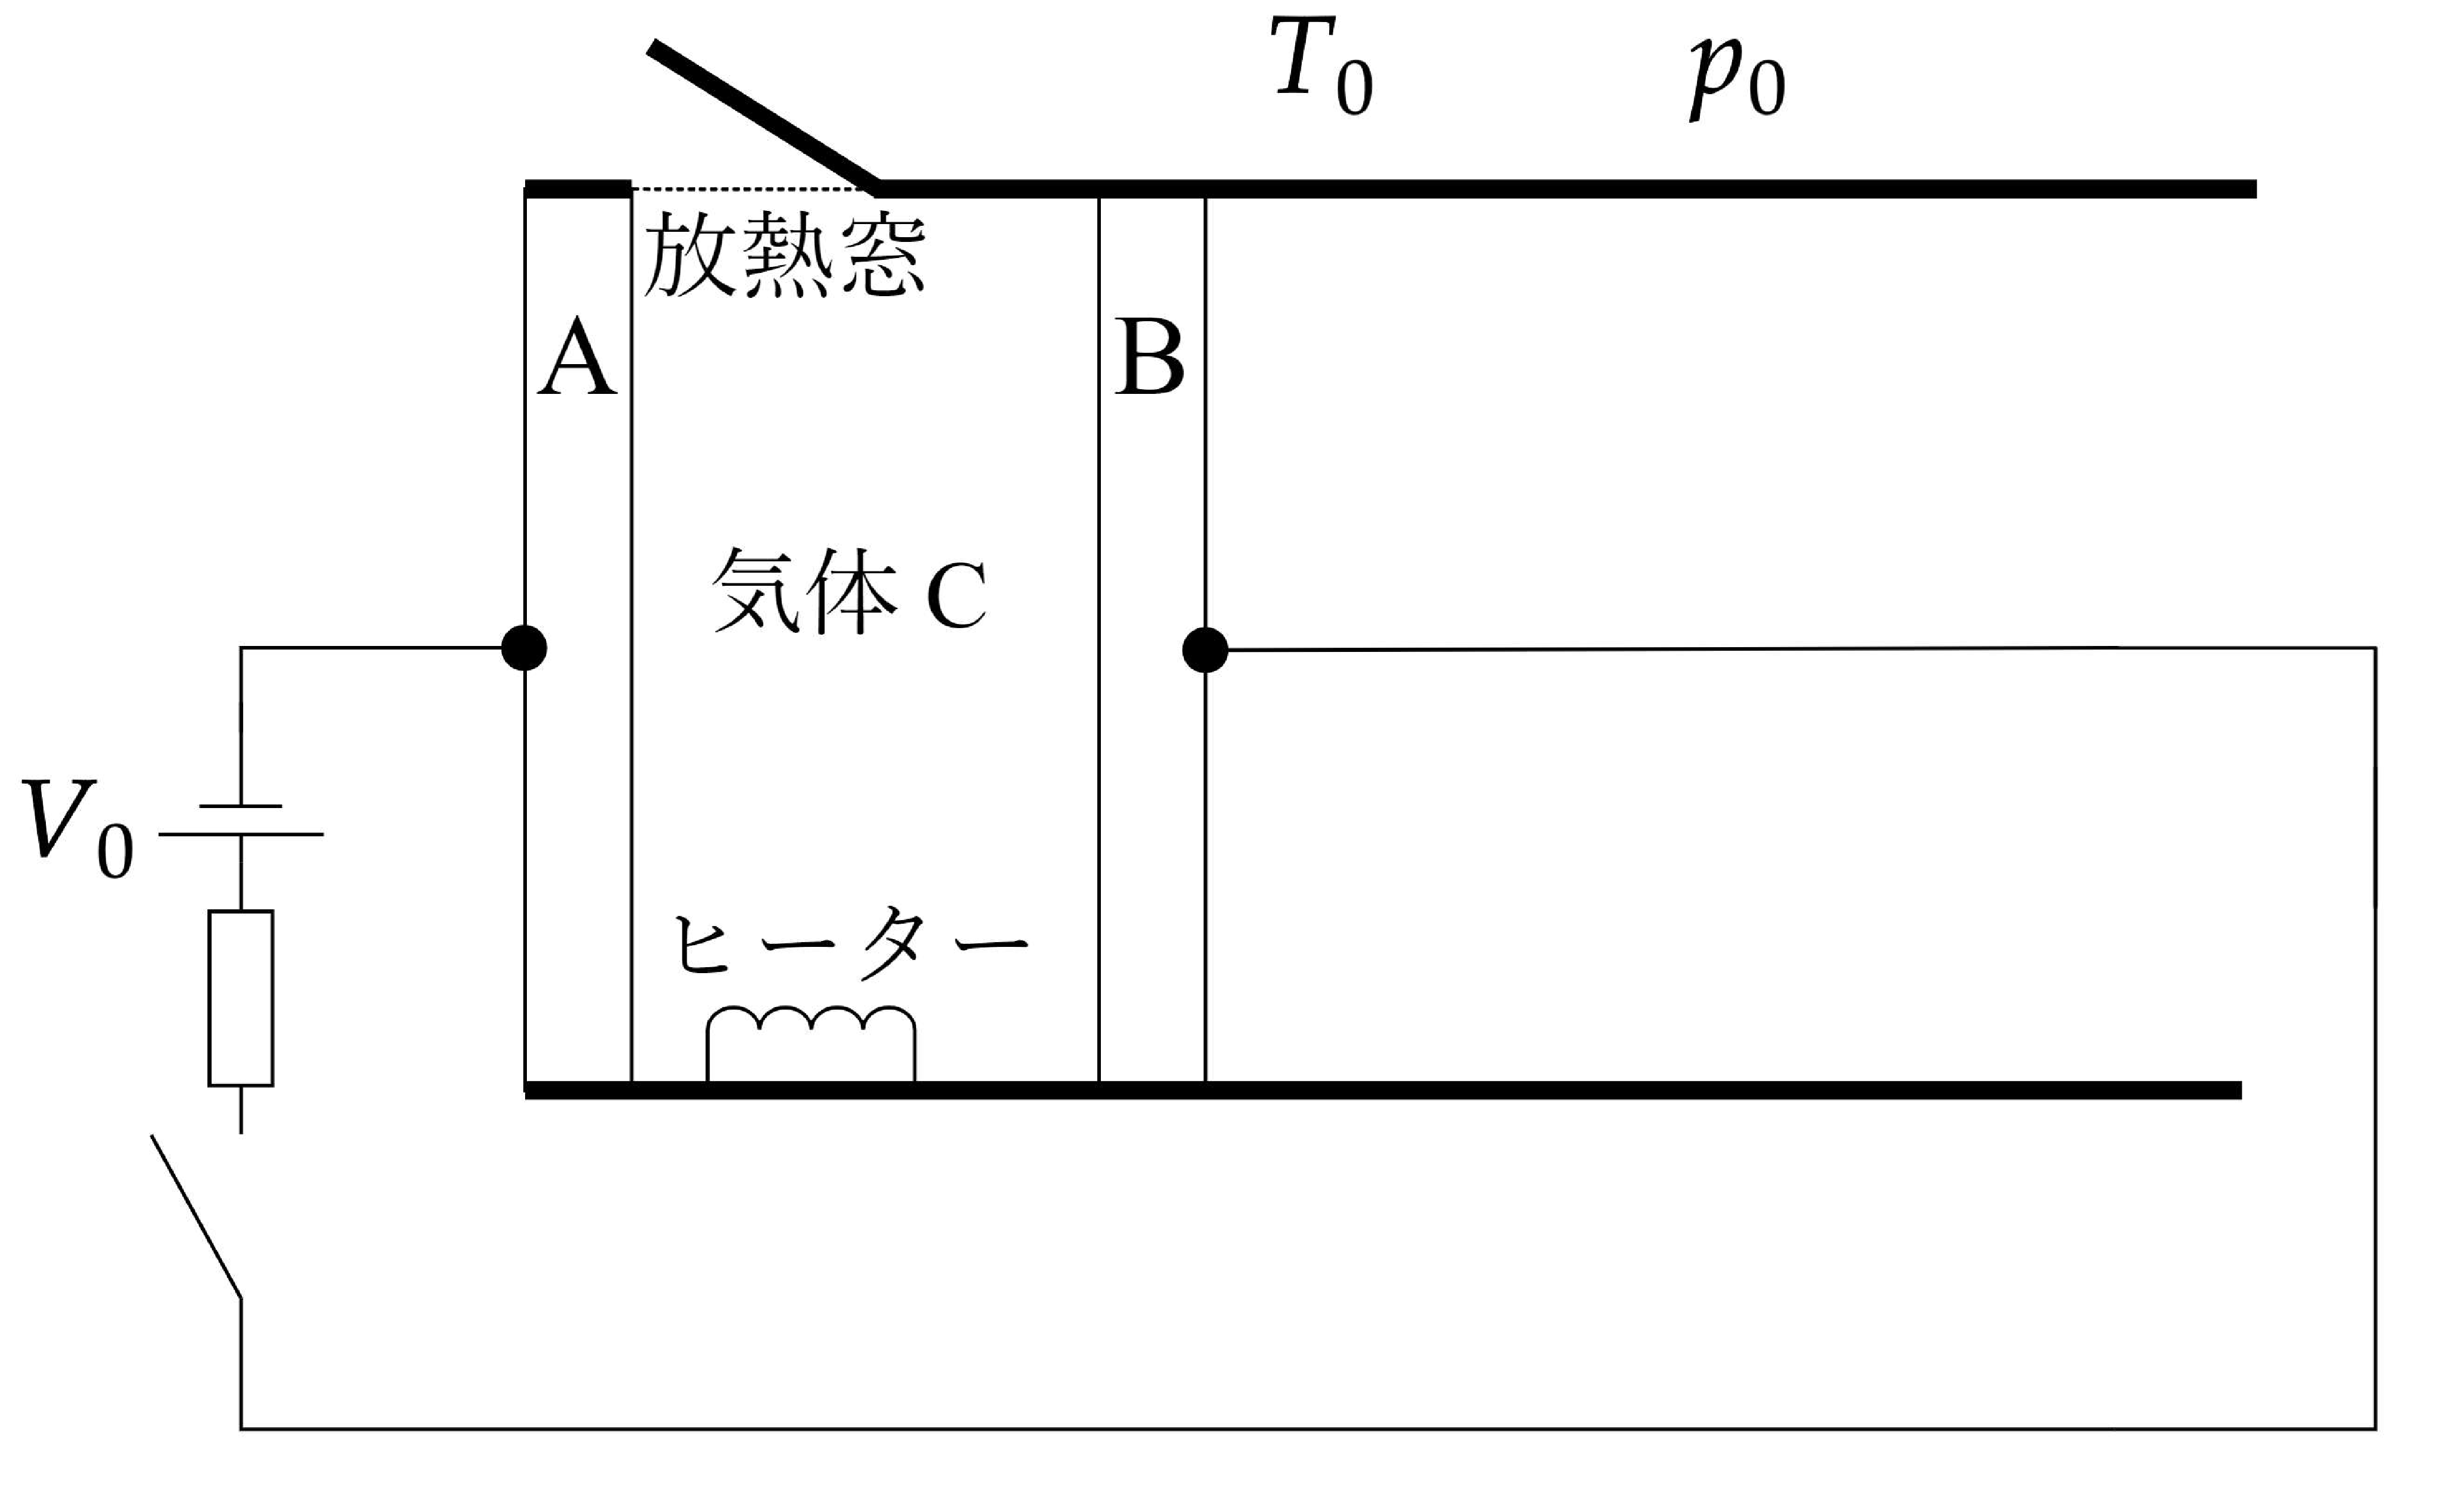
\includegraphics[width=7cm]{fig/fig_4_24.pdf}
\end{wrapfigure}
図のような
 シリンダーに組み込まれたコンデンサーを考える.断面積$S$のシリンダーに2つの導体の極板A,Bが挿入されている.極板A,Bは,図のように導線によって,内部抵抗の無視できる起電力$V_0$の電池,抵抗,スイッチとつながれている.極板Aは固定されていて,極板Bは極板Aと平行を保ったまま,なめらかに動けるようになっており,ピストンの役割をしている.
AとBの間には,$n$〔mol〕の単原子分子理想気体Cが閉じ込められている.
シリンダーの外は圧力$p_0$,温度$T_0$の外気である.シリンダーおよび気体は絶縁体であり,気体の誘電率は$\varepsilon_0$である.
シリンダーには開閉式の放熱窓があり,開いているときには気体Cと外気の間で熱のみを通し,閉じているときには熱を通さない.
シリンダーの他の部分および極板は熱を通さない.また,シリンダー内部にはヒーターがあり,気体Cに熱を加えることができる.
極板,およびシリンダーの熱容量は無視する.
極板間の距離はシリンダーの半径に比べて十分に小さいとする.気体定数を$R$として,以下の問いに答えよ.

まず,スイッチが切れていて放熱窓が開いている場合を考える.気体Cの温度は$T_0$で圧力は$p_0$になっている.極板A,Bは帯電していなかった.このときの極板A,Bの間の距離を$l_0$とする.
\begin{enumerate}[(1)]
  \item $l_0$を,$n$,$R$,$p_0$,$T_0$,$S$のうち必要なものを用いて表せ.
\end{enumerate}

次に,スイッチを切ったまま放熱窓を閉じ,ヒーターで熱を加え,温度が$T$になったところで加熱をやめた.
\begin{enumerate}[(1), resume]
  \item  極板Bが外気に対してした仕事を,$p_0$,$T_0$,$T$,$S$,$l_0$のうち必要なものを用いて表せ. 
  \item この過程でヒーターから加えた熱量を,$n$,$R$,$T_0$,$T$のうち必要なものを用いて表せ.
\end{enumerate}

次に,放熱窓を開き,気体Cの温度が$T_0$になるまで待つ.
その後,スイッチを入れたところ,極板Bは,ゆっくり動いて止まった.
このとき,極板Aに$-q$,極板Bに$+q$ ($q > 0$)の電荷が表れ,極板A,B間の電界(電場)の強さは$E$となった.
\begin{enumerate}[(1), resume]
  \item $E$を$\varepsilon_0$,$q$,$S$,$l_0$のうち必要なものを用いて表せ.
  \item 気体Cの圧力を,$q$,$E$,$p_0$,$S$のうち必要なものを用いて表せ.ただし,極板Bが電界から受ける力の大きさは$\dfrac{qE}{2}$であることに注意せよ.
    これは,極板B上の電荷は,極板A上の電荷$-q$が作る電界$\ab(\text{強さ}\dfrac{E}{2})$のみから力を受けるためである.
  \item 極板A,Bの間の距離を,$q$,$E$,$p_0$,$S$,$l_0$のうち必要なものを用いて表せ.
  \item 電荷$q$を,$\varepsilon_0$,$V_0$,$p_0$,$S$,$l_0$のうち必要なものを用いて表せ.ただし,$V_0 = 0$のときには$q = 0$となることに注意せよ.
  \item スイッチを入れた後,電池がした仕事は$qV_0$である.また,外気は極板Bに対して仕事をしている.これらのエネルギーの行き先として当てはまるものを,次からすべて選び,記号を記せ.
    \begin{enumerate}[label=\mctext{\arabic*}]
      \item 気体Cの内部エネルギーの増加
      \item 放熱窓を通して外気に逃げた熱
      \item 抵抗から発生したジュール熱
    \end{enumerate}
  \item (8)の解答以外のエネルギーの行き先を1つ挙げよ.
\end{enumerate}
 
\end{document}
